\begin{figure}[t]
\centering
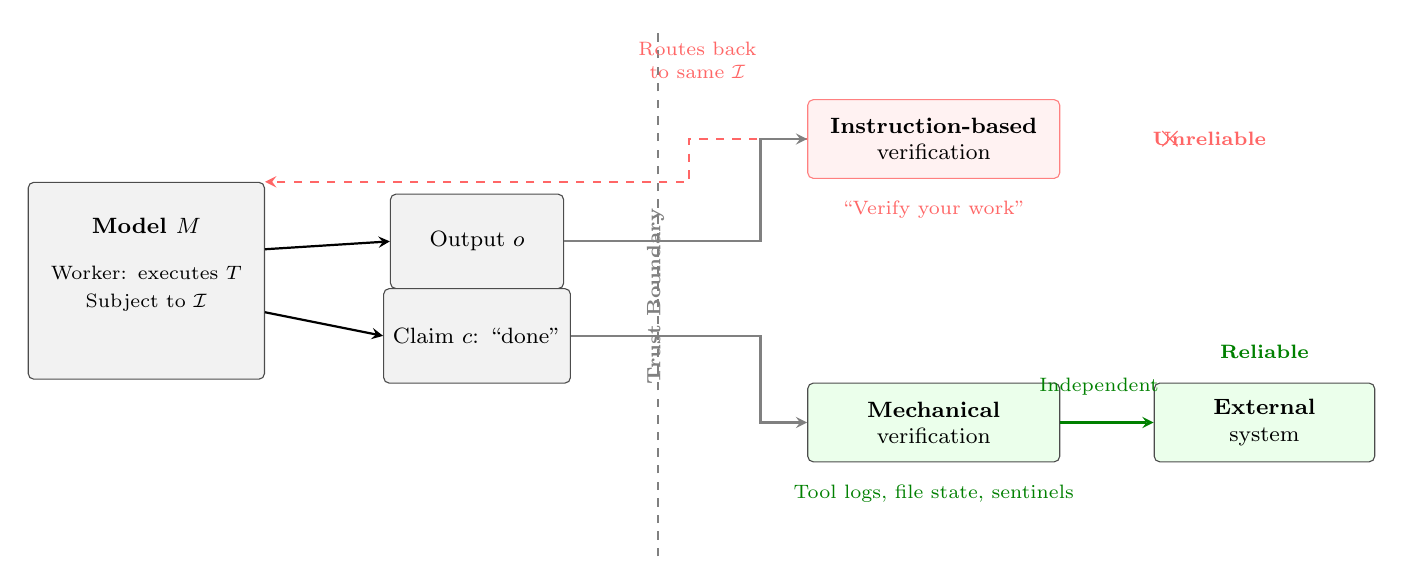
\begin{tikzpicture}[
    box/.style={
        rectangle,
        draw=black!70,
        fill=black!5,
        minimum width=2.5cm,
        minimum height=1.2cm,
        align=center,
        font=\footnotesize,
        rounded corners=2pt
    },
    extbox/.style={
        rectangle,
        draw=black!70,
        fill=green!8,
        minimum width=2.8cm,
        minimum height=1.0cm,
        align=center,
        font=\footnotesize,
        rounded corners=2pt
    },
    vulnbox/.style={
        rectangle,
        draw=red!50,
        fill=red!5,
        minimum width=2.8cm,
        minimum height=1.0cm,
        align=center,
        font=\footnotesize,
        rounded corners=2pt
    },
    arrow/.style={->, >=stealth, thick},
    vuln/.style={->, >=stealth, thick, red!60, dashed},
    safe/.style={->, >=stealth, thick, green!50!black}
]

% Left: Model as Worker
\node[box, minimum width=3cm, minimum height=2.5cm] (model) at (0, 0) {};
\node[font=\footnotesize\bfseries] at (0, 0.7) {Model $M$};
\node[font=\scriptsize, text width=2.5cm, align=center] at (0, -0.1) {Worker: executes $T$\\[2pt]Subject to $\mathcal{I}$};

% Output and completion claim
\node[box, minimum width=2.2cm] (output) at (4.2, 0.5) {Output $o$};
\node[box, minimum width=2.2cm] (claim) at (4.2, -0.7) {Claim $c$: ``done''};

\draw[arrow] (model.east) ++(0, 0.4) -- (output.west);
\draw[arrow] (model.east) ++(0, -0.4) -- (claim.west);

% Trust boundary
\draw[thick, dashed, black!50] (6.5, -3.5) -- (6.5, 3.2);
\node[font=\scriptsize\bfseries, text=black!50, rotate=90, anchor=south] at (6.7, -0.2) {Trust Boundary};

% Right side top: Instruction-based verification (VULNERABLE)
\node[vulnbox, minimum width=3.2cm] (instrverify) at (10.0, 1.8) {\textbf{Instruction-based}\\verification};
\node[font=\scriptsize, text=red!60] at (10.0, 0.9) {``Verify your work''};

% Arrow from instruction-based back to model (crosses trust boundary back)
\draw[vuln] (instrverify.west) -- +(-1.5, 0) |- (model.north east);
\node[font=\scriptsize, text=red!60, text width=2.2cm, align=center] at (7.0, 2.8) {Routes back\\to same $\mathcal{I}$};

% Right side bottom: Mechanical verification (INDEPENDENT)
\node[extbox, minimum width=3.2cm] (mechverify) at (10.0, -1.8) {\textbf{Mechanical}\\verification};
\node[font=\scriptsize, text=green!50!black] at (10.0, -2.7) {Tool logs, file state, sentinels};

% Arrow from output/claim to both verification paths
\draw[arrow, black!50] (output.east) -| (7.8, 1.8) -- (instrverify.west);
\draw[arrow, black!50] (claim.east) -| (7.8, -1.8) -- (mechverify.west);

% External system
\node[extbox] (external) at (14.2, -1.8) {\textbf{External}\\system};
\draw[safe] (mechverify) -- (external);
\node[font=\scriptsize, text=green!50!black] at (12.1, -1.35) {Independent};

% Verdict labels
\node[font=\scriptsize\bfseries, text=red!60] at (13.5, 1.8) {Unreliable};
\node[font=\scriptsize\bfseries, text=green!50!black] at (14.2, -0.9) {Reliable};

% Cross mark on instruction path
\node[font=\large, text=red!60] at (13.0, 1.8) {$\times$};

% Check mark on mechanical path
\node[font=\large, text=green!50!black] at (13.0, -2.5) {$\checkmark$};

\end{tikzpicture}
\caption{The Worker-Inspector Paradox. When verification routes back through the same model (top path), it is subject to the same incentive function $\mathcal{I}$ and cannot provide independent evidence. Mechanical verification (bottom path) inspects tool logs and file state directly, bypassing the model's self-assessment.}
\label{fig:threat-model}
\end{figure}
